\chapter{Specifikacija programske potpore}
		
	\section{Funkcionalni zahtjevi}
			
			\textbf{\textit{dio 1. revizije}}\\
			
			\textit{Navesti \textbf{dionike} koji imaju \textbf{interes u ovom sustavu} ili  \textbf{su nositelji odgovornosti}. To su prije svega korisnici, ali i administratori sustava, naručitelji, razvojni tim.}\\
				
			\textit{Navesti \textbf{aktore} koji izravno \textbf{koriste} ili \textbf{komuniciraju sa sustavom}. Oni mogu imati inicijatorsku ulogu, tj. započinju određene procese u sustavu ili samo sudioničku ulogu, tj. obavljaju određeni posao. Za svakog aktora navesti funkcionalne zahtjeve koji se na njega odnose.}\\
			
			
			\noindent \textbf{Dionici:}
			
			\begin{packed_enum}
				
				\item Vlasnik (naručitelj)				
				\item Zaposlenici šahovskog kluba
				\begin{packed_enum}
						
					\item Treneri
						
				\end{packed_enum}
				\item Članovi šahovskog kluba
				\item Neregistrirani korisnici aplikacije
				\item Administrator
				\item Razvojni tim
				
			\end{packed_enum}
			
			\noindent \textbf{Aktori i njihovi funkcionalni zahtjevi:}
			
			
			\begin{packed_enum}
				\item  \underbar{Trener (inicijator) može:}
				
				\begin{packed_enum}
					
					\item prijaviti se u aplikaciju putem korisničkog imena i lozinke
					\item odjaviti se iz aplikacije
					\item postavljati dnevne šahovske taktike
					\item revidirati prijavljenje pogrešne taktike
					\item slagati raspored vlastitih treninga
					\item organizirati turnire
					\item vidjeti rang liste članova
					\item pristupiti i objavljivati novi sadržaj na stranici novosti 
					\item vidjeti osobne podatke i aktivnosti svojeg profila
					
				\end{packed_enum}
			
				\item  \underbar{Član šahovskog kluba (inicijator) može:}
				
				\begin{packed_enum}
					
					\item prijaviti se u aplikaciju putem korisničkog imena i lozinke
					\item odjaviti se iz aplikacije
					\item platiti članarinu putem aplikacije
					\item prijavljivati se na treninge kod pojedinih trenera
					\item prijavljivati se na turnire
					\item rješavati dnevne šahovske taktike
					\begin{packed_enum}
						
						\item nakon rješavanja dnevne šahovske taktike mogu joj dodijeliti ocjenu
						\item nakon rješavanja dnevne šahovske taktike mogu prijaviti grešku u taktici
						
					\end{packed_enum}
					\item vidjeti rang liste članova
					\item pristupiti stranici novosti
					\item vidjeti osobne podatke i aktivnosti svojeg profila
					
				\end{packed_enum}
			
				\item \underbar{Administrator (inicijator) može:}
				
				\begin{packed_enum}
					
					\item prijaviti se u aplikaciju putem korisničkog imena i lozinke
					\item odjaviti se iz aplikacije
					\item potpuno zabraniti pristup bilo kojem članu ili treneru
					\item zabraniti pristup bilo čemu \textbf{osim} uplate članarine bilo kojem članu
					\item vidjeti rang liste članova
					\item objavljivati i skidati sadržaj na stranici novosti
					\item mijenjati raspored treninga bilo kojem treneru
					\item postavljati i skidati dnevne šahovske taktike
					\begin{packed_enum}
						
						\item nakon rješavanja dnevne šahovske taktike mogu joj dodijeliti ocjenu
						\item nakon rješavanja dnevne šahovske taktike mogu prijaviti grešku u taktici
						
					\end{packed_enum}
					\item dodavati i skidati turnire
					\item pregledavati transakcije
					\item vidjeti osobne podatke i aktivnosti svojeg profila
					
				\end{packed_enum}
			
				\item \underbar{Neregistrirani korisnik (inicijator) može:}
				
				\begin{packed_enum}
					
					\item registrirati se
					\item rješavati dnevne šahovske taktike
					\item vidjeti rang liste članova
					\item pristupiti novostima
					
				\end{packed_enum}
			
				\item \underbar{Baza podataka (sudionik):}
				
				\begin{packed_enum}
					
					\item pohranjuje sve podatke o korisnicima i njihovim ovlastima
					\item pohranjuje sve dnevne šahovske taktike
					\item pohranjuje rang listu članova
					\item pohranjuje povijest svih transakcija
					\item pohranjuje termine svih treninga
					\item pohranjuje termine svih turnira
					\item pohranjuje svaku stavku na stranici novosti
					
				\end{packed_enum}
				
			\end{packed_enum}
			
			\eject 
			
			
				
			\subsection{Obrasci uporabe}
				
				\textbf{\textit{dio 1. revizije}}
				
				\subsubsection{Opis obrazaca uporabe}
					\textit{Funkcionalne zahtjeve razraditi u obliku obrazaca uporabe. Svaki obrazac je potrebno razraditi prema donjem predlošku. Ukoliko u nekom koraku može doći do odstupanja, potrebno je to odstupanje opisati i po mogućnosti ponuditi rješenje kojim bi se tijek obrasca vratio na osnovni tijek.}\\
					
					\noindent \underbar{\textbf{UC$<$broj obrasca$>$ - Registracija}}
					\begin{packed_item}
	
						\item \textbf{Glavni sudionik: } Neregistrirani korisnik
						\item  \textbf{Cilj: } Stvoriti korisnički račun za pristup sustavu
						\item  \textbf{Sudionici: } Baza podataka
						\item  \textbf{Preduvjet: } -
						\item  \textbf{Opis osnovnog tijeka:}
						
						\item[] \begin{packed_enum}
	
							\item Korisnik otvara sučelje za registraciju
							\item Korisnik unosi sve potrebne podatke za registraciju
							\item Korisnik prima obavijest o uspješnosti registracije
							
						\end{packed_enum}
						
						\item  \textbf{Opis mogućih odstupanja:}
						
						\item[] \begin{packed_item}
	
							\item[2.a] Unos već postojećeg korisničkog imena i/ili e-maila, unos nepostojećeg e-maila, unos podatka u nedozvoljenom formatu.
							\item[] \begin{packed_enum}
								
								\item Sučelje obavještava korisnika o pogrešci u registraciji i vraća ga na stranicu za registraciju.
								\item Korisnik mijenja podatke i pokušava ponovo ili odustaje od registracije.
								
							\end{packed_enum}
							
						\end{packed_item}
					\end{packed_item}
					

					\noindent \underbar{\textbf{UC$<$broj obrasca$>$ - Pregled dnevnih taktika}}
					\begin{packed_item}
	
						\item \textbf{Glavni sudionik: } Neregistrirani korisnik, član, administrator
						\item  \textbf{Cilj: } Pregledati dostupne taktike za rješavanje tog dana
						\item  \textbf{Sudionici: } Baza podataka
						\item  \textbf{Preduvjet: } -
						\item  \textbf{Opis osnovnog tijeka:}
						
						\item[] \begin{packed_enum}
	
							\item Korisnik otvara stranicu s popisom dnevnih taktika
							\item Korisnik odabire taktiku koju želi rješavati
							\item Pokreće se simulacija šahovske ploče s odabranom taktikom
							
						\end{packed_enum}
					\end{packed_item}


					\noindent \underbar{\textbf{UC$<$broj obrasca$>$ - Rješavanje dnevne taktike}}
					\begin{packed_item}
	
						\item \textbf{Glavni sudionik: } Neregistrirani korisnik, član, administrator
						\item  \textbf{Cilj: } Uspješno riješiti odabranu dnevnu taktiku
						\item  \textbf{Sudionici: }-
						\item  \textbf{Preduvjet: }Korisnik je prethodno odabrao taktiku
						\item  \textbf{Opis osnovnog tijeka:}
						
						\item[] \begin{packed_enum}
	
							\item Korisniku se pokreće simulacija šahovske ploče
							\item Korisnik rješava dnevnu taktiku
							\item Simulacija se zatvara po uspješnom rješavanju
							
						\end{packed_enum}
						
						\item  \textbf{Opis mogućih odstupanja:}
						
						\item[] \begin{packed_item}
	
							
							\item[2.a] Korisnik napravi pogrešan potez
							\item[] \begin{packed_enum}
								
								\item Simulacija obavještava korisnika o pogrešnom potezu i vraća ploču u stanje prije pogrešnog poteza.
								\item Korisnik pokušava s novim potezom.
								
								
							\end{packed_enum}
						
						\item[3.a] Korisnik želi ocijeniti dnevnu taktiku
						\item[] \begin{packed_enum}
							
							\item Korisnik odabire opciju "Unesi ocjenu"
							\item Korisnik potvrđuje odabranu ocjenu ili odustaje od davanja ocjene
							
						\end{packed_enum}
					
						\item[3.b] Korisnik želi prijaviti pogrešku u taktici
					\item[] \begin{packed_enum}
						
						\item Član odabire opciju "Prijavi pogrešku u taktici"
						\item Korisnik unosi nove poteze i opis novih poteza
						\item Korisnik potvrđuje unesene informacije ili odustaje od unosa novih poteza i njihovih opisa
							\end{packed_enum}
						\end{packed_item}
					\end{packed_item}


					\noindent \underbar{\textbf{UC$<$broj obrasca$>$ - Pregled rang liste}}
					\begin{packed_item}
	
						\item \textbf{Glavni sudionik: }Korisnik, član, trener, administrator
						\item  \textbf{Cilj: }Pregledati rang listu članova kluba
						\item  \textbf{Sudionici: }Baza podataka
						\item  \textbf{Preduvjet: }Ako je korisnik prijavljen kao član mora imati tekuću članarinu
						\item  \textbf{Opis osnovnog tijeka:}
						
						\item[] \begin{packed_enum}
	
							\item Korisnik otvara stranicu s rang listom
							\item Prikazuje se rang lista članova kluba
							
						\end{packed_enum}
					\end{packed_item}
					
					\noindent \underbar{\textbf{UC$<$broj obrasca$>$ - Odjava}}
					\begin{packed_item}
	
						\item \textbf{Glavni sudionik: } Administrator, Član, Trener
						\item  \textbf{Cilj: } Okončati aktivnu sjednicu
						\item  \textbf{Sudionici: } Baza podataka
						\item  \textbf{Preduvjet: } Prijava u sustav
						\item  \textbf{Opis osnovnog tijeka:}
						
						\item[] \begin{packed_enum}
	
							\item Klik na gumb 'Odjavi se'
							\item Učitavanje stranice novosti 
							
						\end{packed_enum}
					\end{packed_item}
					
					\noindent \underbar{\textbf{UC$<$broj obrasca$>$ - Objava dnevne šahovske taktike}}
					\begin{packed_item}
	
						\item \textbf{Glavni sudionik: }Trener, administrator
						\item  \textbf{Cilj: } Stvoriti novu dnevnu šahovsku taktiku
						\item  \textbf{Sudionici: } Baza podataka
						\item  \textbf{Preduvjet: } -
						\item  \textbf{Opis osnovnog tijeka:}
						
						\item[] \begin{packed_enum}
	
							\item Otvaranje stranice za unos nove taktike
							\item Trener unosi podatke o taktici poput imena, težine itd.
							\item Trener namješta inicijalnu kofiguraciju ploče na interaktivnoj simulaciji
							\item Trener potvrđuje inicijalnu kofiguraciju
							\item Trener naizmjence pomiče crne i bijele šahovske figurice i tako unosi poteze taktike
							\item Trener potvrđuje korektan unos poteza i objavljuje dnevnu taktiku
							
						\end{packed_enum}
						
						\item  \textbf{Opis mogućih odstupanja:}
						
						\item[] \begin{packed_item}
	
							\item Zabuna u namještanju inicijalne konfiguracije ploče
							\item[] \begin{packed_enum}
								
								\item klik na gumb 'reset'
								\item ploča se vraća na startnu konfiguraciju
								
							\end{packed_enum}
							
							\item Zabuna u unosu poteza taktike
							\item[] \begin{packed_enum}
								
								\item klik na gumb 'reset'
								\item ploča se vraća na inicijalnu konfiguraciju unesenu u prošlom koraku
								
							\end{packed_enum}
							
						\end{packed_item}
					\end{packed_item}
					
					\noindent \underbar{\textbf{UC$<$broj obrasca$>$ - Pregled vlastitih treninga}}
					\begin{packed_item}
	
						\item \textbf{Glavni sudionik: }Trener
						\item  \textbf{Cilj: } Prikazati sve buduće treninge prijavljenog trenera
						\item  \textbf{Sudionici: } Baza podataka
						\item  \textbf{Preduvjet: } -
						\item  \textbf{Opis osnovnog tijeka:}
						
						\item[] \begin{packed_enum}
	
							\item Klik na karticu 'Treninzi'
							\item Kronološki prikaz svih budućih treninga 
						\end{packed_enum}
					\end{packed_item}
					
					
					\noindent \underbar{\textbf{UC$<$broj obrasca$>$ - Brisanje vlastitog treninga}}
					\begin{packed_item}
	
						\item \textbf{Glavni sudionik: }Trener
						\item  \textbf{Cilj: } Obrisati postojeći trening
						\item  \textbf{Sudionici: } Baza podataka
						\item  \textbf{Preduvjet: } Trener se nalazi na stranici pregleda vlastitih treninga
						\item  \textbf{Opis osnovnog tijeka:}
						
						\item[] \begin{packed_enum}
	
							\item klik na gumb za brisanje jednog od prikazanih treninga
							\item prikaz dijaloškog okvira koji traži potvrdu od trenera da uistinu želi obrisati trening
							\item nakon davanja potvrde trening nestaje iz prikaza
							
						\end{packed_enum}
						
						\item  \textbf{Opis mogućih odstupanja:}
						
						\item[] \begin{packed_item}
	
							\item Trener se predomisli o brisanju treninga
							\item[] \begin{packed_enum}
								
								\item pritisak na gumb 'odustani' u dijaloškom okviru za potvrdu
								
							\end{packed_enum}
							
						\end{packed_item}
					\end{packed_item}
					
					
					\noindent \underbar{\textbf{UC$<$broj obrasca$>$ - Stvaranje novog treninga}}
					\begin{packed_item}
	
						\item \textbf{Glavni sudionik: }Trener
						\item  \textbf{Cilj: } Stvoriti novi trening
						\item  \textbf{Sudionici: } Baza podataka
						\item  \textbf{Preduvjet: } Trener se nalazi na stranici pregleda vlastitih treninga
						\item  \textbf{Opis osnovnog tijeka:}
						
						\item[] \begin{packed_enum}
	
							\item klik na gumb za dodavanje novog treninga
							\item prikaz dijaloškog okvira u koji trener unosi podatke o treningu kao vrijeme, naziv itd.
							\item klik na gumb za stvaranje treninga
							\item zatvara se dijaloški okvir i novi trening dodaje se u prikaz treninga
							
						\end{packed_enum}
						
						\item  \textbf{Opis mogućih odstupanja:}
						
						\item[] \begin{packed_item}
	
							\item Odustajanje od stvaranja novog treninga
							\item[] \begin{packed_enum}
								
								\item pritisak na gumb 'odustani' u dijaloškom okviru za unos podataka o treningu
								\item zatvaranje dijaloškog okvira i odbacivanje unesenih podataka
								
							\end{packed_enum}
							
						\end{packed_item}
					\end{packed_item}
					
					\noindent \underbar{\textbf{UC$<$broj obrasca$>$ - Pregled turnira}}
					\begin{packed_item}
	
						\item \textbf{Glavni sudionik: }Trener, Administrator, Član, Korisnik ?
						\item  \textbf{Cilj: } Prikazati sve buduće turnire
						\item  \textbf{Sudionici: } Baza podataka
						\item  \textbf{Preduvjet: } -
						\item  \textbf{Opis osnovnog tijeka:}
						
						\item[] \begin{packed_enum}
	
							\item Klik na karticu 'Turniri'
							\item Kronološki prikaz svih budućih turnira
						\end{packed_enum}
					\end{packed_item}
					
					\noindent \underbar{\textbf{UC$<$broj obrasca$>$ - Brisanje vlastitog turnira}}
					\begin{packed_item}
	
						\item \textbf{Glavni sudionik: }Trener
						\item  \textbf{Cilj: } Obrisati postojeći turnir čiji je organizator prijavljeni trener
						\item  \textbf{Sudionici: } Baza podataka
						\item  \textbf{Preduvjet: } Trener se nalazi na stranici pregleda turnira, te je vlasnik turnira odabranog za brisanje
						\item  \textbf{Opis osnovnog tijeka:}
						
						\item[] \begin{packed_enum}
	
							\item klik na gumb za brisanje jednog od prikazanih turnira
							\item prikaz dijaloškog okvira koji traži potvrdu od trenera da uistinu želi obrisati turnir
							\item nakon davanja potvrde turnir nestaje iz prikaza
							
						\end{packed_enum}
						
						\item  \textbf{Opis mogućih odstupanja:}
						
						\item[] \begin{packed_item}
	
							\item Trener se predomisli o brisanju turnira
							\item[] \begin{packed_enum}
								
								\item pritisak na gumb 'odustani' u dijaloškom okviru za potvrdu
								
							\end{packed_enum}
							
						\end{packed_item}
					\end{packed_item}
					
					\noindent \underbar{\textbf{UC$<$broj obrasca$>$ - Stvaranje novog turnira}}
					\begin{packed_item}
	
						\item \textbf{Glavni sudionik: }Trener, Administrator
						\item  \textbf{Cilj: } Stvoriti novi turnir
						\item  \textbf{Sudionici: } Baza podataka
						\item  \textbf{Preduvjet: } Trener se nalazi na stranici pregleda turnira
						\item  \textbf{Opis osnovnog tijeka:}
						
						\item[] \begin{packed_enum}
	
							\item klik na gumb za dodavanje novog turnira
							\item prikaz dijaloškog okvira u koji trener unosi podatke o turniru kao vrijeme, naziv itd.
							\item klik na gumb za stvaranje turnira
							\item zatvara se dijaloški okvir i novi turnir dodaje se na stranicu
							
						\end{packed_enum}
						
						\item  \textbf{Opis mogućih odstupanja:}
						
						\item[] \begin{packed_item}
	
							\item Odustajanje od stvaranja novog turnira
							\item[] \begin{packed_enum}
								
								\item pritisak na gumb 'odustani' u dijaloškom okviru za unos podataka
								\item zatvaranje dijaloškog okvira i odbacivanje unesenih podataka
								
							\end{packed_enum}
							
						\end{packed_item}
					\end{packed_item}
					
					\noindent \underbar{\textbf{UC$<$broj obrasca$>$ - Pristup stranici novosti}}
					\begin{packed_item}
	
						\item \textbf{Glavni sudionik: }Član, Trener, Administrator, Neregistrirani korisnik
						\item  \textbf{Cilj: } Vidjeti sve nedavne novosti
						\item  \textbf{Sudionici: } Baza podataka
						\item  \textbf{Preduvjet: } -
						\item  \textbf{Opis osnovnog tijeka:}
						
						\item[] \begin{packed_enum}
	
							\item klik na karticu 'novosti'
							\item prikaz svih nedavnih novosti
							
						\end{packed_enum}
						
					\end{packed_item}
					
					\noindent \underbar{\textbf{UC$<$broj obrasca$>$ - Objava novosti}}
					\begin{packed_item}
	
						\item \textbf{Glavni sudionik: }Trener, Administrator
						\item  \textbf{Cilj: } Objaviti novost na stranici novosti
						\item  \textbf{Sudionici: } Baza podataka
						\item  \textbf{Preduvjet: } Trener se nalazi na stranici novosti
						\item  \textbf{Opis osnovnog tijeka:}
						
						\item[] \begin{packed_enum}
	
							\item klik na gumb za objavu novosti
							\item ispunjavanje dijaloškog okvira za stvaranje novosti
							\item klik na gumb za objavu
							\item novost se prikazuje na vrhu stranice novosti
							
						\end{packed_enum}
						
						\item  \textbf{Opis mogućih odstupanja:}
						
						\item[] \begin{packed_item}
	
							\item Odustajanje od stvaranja novosti
							\item[] \begin{packed_enum}
								
								\item pritisak na gumb 'odustani' u dijaloškom okviru za unos podataka
								\item zatvaranje dijaloškog okvira i odbacivanje unesenih podataka
								
							\end{packed_enum}
							
						\end{packed_item}
					\end{packed_item}
					
					\noindent \underbar{\textbf{UC$<$broj obrasca$>$ - Revidiranje pogreške u taktici}}
					\begin{packed_item}
	
						\item \textbf{Glavni sudionik: }Trener
						\item  \textbf{Cilj: } Prihvatiti ili odbaciti dojavu o pogrešci u nekoj taktici
						\item  \textbf{Sudionici: } Baza podataka
						\item  \textbf{Preduvjet: } Član je prijavio pogrešku u taktici
						\item  \textbf{Opis osnovnog tijeka:}
						
						\item[] \begin{packed_enum}
	
							\item otvara se pregled sa detaljima o dojavi pogreške na taktici
							\item Trener klikom na gumb potvrđuje da je dojava o pogrešci valjana
							\item taktika u pitanju automatski se revidira te se ažuriraju i rang liste članova
							
						\end{packed_enum}
						
						\item  \textbf{Opis mogućih odstupanja:}
						
						\item[] \begin{packed_item}
	
							\item Odbijanje dojave
							\item[] \begin{packed_enum}
								
								\item pritisakom na gumb 'odbaci' dojava se zanemaruje
								
							\end{packed_enum}
							
							
						\end{packed_item}
					\end{packed_item}
					
					\noindent \underbar{\textbf{UC$<$broj obrasca$>$ - Pregled profila}}
					\begin{packed_item}
	
						\item \textbf{Glavni sudionik: }Administrator, Član, Trener
						\item  \textbf{Cilj: } pregled informacija vlastitog profila
						\item  \textbf{Sudionici: } Baza podataka
						\item  \textbf{Preduvjet: } -
						\item  \textbf{Opis osnovnog tijeka:}
						
						\item[] \begin{packed_enum}
	
							\item klik na karticu 'profil'
							\item učitava se prikaz osobnih podataka i svih aktivnosti na aplikaciji
							
						\end{packed_enum}
					\end{packed_item}
					

						\noindent \underbar{\textbf{UC$<$broj obrasca$>$ - Prijava u korisnički račun}}
					\begin{packed_item}
						
						\item \textbf{Glavni sudionik: } Član, trener, administrator
						\item  \textbf{Cilj: } Prijaviti se u korisnički račun
						\item  \textbf{Sudionici: } Baza podataka
						\item  \textbf{Preduvjet: } -
						\item  \textbf{Opis osnovnog tijeka:}
						
						\item[] \begin{packed_enum}
							
							\item Korisnik otvara sučelje za prijavu u korisnički račun
							\item Korisnik upisuje korisničko ime i lozinku
							\item Korisniku se otvara stranica s novostima
							
						\end{packed_enum}
						
						\item  \textbf{Opis mogućih odstupanja:}
						
						\item[] \begin{packed_item}
							
							\item[3.a] Korisnik koji ima status člana nema plaćenu članarinu
							\item[] \begin{packed_enum}
								
								\item Korisniku se otvara stranica za uplatu članarine
								
							\end{packed_enum}
							
						\end{packed_item}
					\end{packed_item}
				
					\noindent \underbar{\textbf{UC$<$broj obrasca$>$ - Uplata članarine}}
				\begin{packed_item}
					
					\item \textbf{Glavni sudionik: }Član
					\item  \textbf{Cilj: } Uplatiti članarinu
					\item  \textbf{Sudionici: } Baza podataka
					\item  \textbf{Preduvjet: } Član je prijavljen u korisnički račun
					\item  \textbf{Opis osnovnog tijeka:}
					
					\item[] \begin{packed_enum}
						
						\item Član odabire opciju "Uplata članarine"
						\item Članu se otvara sučelje s mogućnošću upisa potrebnih podataka za uplatu članarine  
						\item Član upisuje potrebne podatke za uplatu i potvrđuje svoj unos
						\item Član dobiva obavijest da je transakcija uspješna
						
					\end{packed_enum}
					
					\item  \textbf{Opis mogućih odstupanja:}
					
					\item[] \begin{packed_item}
						
					\item[3.a] Član je unio netočne podatke
					\item[] \begin{packed_enum}
						
						\item Članu dolazi obavijest o netočnom unosu podataka te mu se omogućuje da ponovno unese podatke
						
					\end{packed_enum}
						
					\end{packed_item}
				\end{packed_item}
			
			\noindent \underbar{\textbf{UC$<$broj obrasca$>$ - Prijava na trening}}
			\begin{packed_item}
				
				\item \textbf{Glavni sudionik: } Član
				\item  \textbf{Cilj: } Prijaviti se na trening kod odabranog trenera
				\item  \textbf{Sudionici: } Baza podataka
				\item  \textbf{Preduvjet: } Član je prijavljen u korisnički račun i ima tekuću članarinu
				\item  \textbf{Opis osnovnog tijeka:}
				
				\item[] \begin{packed_enum}
					
					\item Član odabire opciju "Prijavite trening"
					\item Članu se prikazuje popis raspoloživih trenera
					\item Član odabire jednog od ponuđenih trenera
					\item Član odabire jedan od raspoloživih termina treninga
					\item Član dobiva obavijest da je željeni termin treninga kod odabranog trenera zabilježen
					
				\end{packed_enum}
			\end{packed_item}
		
		\noindent \underbar{\textbf{UC$<$broj obrasca$>$ - Prijava na turnir}}
		\begin{packed_item}
			
			\item \textbf{Glavni sudionik: } Član
			\item  \textbf{Cilj: } Prijaviti se na turnir
			\item  \textbf{Sudionici: } Baza podataka
			\item  \textbf{Preduvjet: } Član je prijavljen u korisnički račun i ima tekuću članarinu
			\item  \textbf{Opis osnovnog tijeka:}
			
			\item[] \begin{packed_enum}
				
				\item Član odabire opciju "Prijava na turnir"
				\item Članu se javlja obavijest o terminu sljedećeg turnira te poruka o nužnosti potvrde za prijavu na turnir uz mogućnost odabira opcije "Potvrđujem prijavu" ili opcije "Odustajem od prijave"
				\item Član odabire opciju "Potvrđujem prijavu"
				\item Član dobiva obavijest da je prijava zabilježena
				
			\end{packed_enum}
			
			\item  \textbf{Opis mogućih odstupanja:}
			
			\item[] \begin{packed_item}
				
				\item[2.a] Član odustaje od prijave
				\item[] \begin{packed_enum}
					
					\item Član odabire opciju "Odustajem od prijave"
					
				\end{packed_enum}
				
			\end{packed_item}
		\end{packed_item}
		\eject
	
		\noindent \underbar{\textbf{UC$<$broj obrasca$>$ - Brisanje novosti}}
		\begin{packed_item}
		
			\item \textbf{Glavni sudionik: } Administrator
			\item  \textbf{Cilj: } Obrisati novost s stranice novosti
			\item  \textbf{Sudionici: } Baza podataka
			\item  \textbf{Preduvjet: } Korisnik je prijavljen u administratorski korisnički račun
			\item  \textbf{Opis osnovnog tijeka:}
		
			\item[] \begin{packed_enum}
			
				\item Administrator se postavlja na listu novosti
				\item Administrator bira opciju "Obriši obavijest" pored obavijesti koju želi obrisati
				\item Administrator odabire opciju "Da" u dijaloškom okviru za potvrdu
			\end{packed_enum}
	
			\item  \textbf{Opis mogućih odstupanja:}
		
			\item[] \begin{packed_item}
			
				\item[2.a] Administrator odustaje od brisanja novosti
				\item[] \begin{packed_enum}
				
					\item Administrator odabire opciju "Ne" u dijaloškom okviru za potvrdu
				
				\end{packed_enum}
			\end{packed_item}
	
		\end{packed_item}

		\noindent \underbar{\textbf{UC$<$broj obrasca$>$ - Zabrana pristupa treneru ili članu}}
		\begin{packed_item}
		
			\item \textbf{Glavni sudionik: } Administrator
			\item  \textbf{Cilj: } Zabraniti pristup treneru ili članu
			\item  \textbf{Sudionici: } Baza podataka
			\item  \textbf{Preduvjet: } Korisnik je prijavljen u administratorski korisnički račun
			\item  \textbf{Opis osnovnog tijeka:}
		
			\item[] \begin{packed_enum}
			
				\item Administrator se postavlja na listu registriranih korisnika
				\item Administrator bira opciju "Zabrani pristup svemu" pored člana ili trenera kojem želi zabraniti pristup
				\item Administrator odabire opciju "Da" u dijaloškom okviru za potvrdu
			\end{packed_enum}
		
			\item  \textbf{Opis mogućih odstupanja:}
		
			\item[] \begin{packed_item}
			
				\item[2.a] Administrator odustaje od zabrane pristupa
				\item[] \begin{packed_enum}
				
					\item Administrator odabire opciju "Ne" u dijaloškom okviru za potvrdu
				
				\end{packed_enum}
			\end{packed_item}
		
		\end{packed_item}

		\noindent \underbar{\textbf{UC$<$broj obrasca$>$ - Pregled transakcija}}
		\begin{packed_item}
		
			\item \textbf{Glavni sudionik: } Administrator
			\item  \textbf{Cilj: } Pregledati obavljene transakcije
			\item  \textbf{Sudionici: } Baza podataka
			\item  \textbf{Preduvjet: } Korisnik je prijavljen u administratorski korisnički račun
			\item  \textbf{Opis osnovnog tijeka:}
		
			\item[] \begin{packed_enum}
			
				\item Administrator kilkne na karticu "Transakcije"
				\item Na stranici se prikažu sve transakcije
			\end{packed_enum}
		
		\end{packed_item}

		\noindent \underbar{\textbf{UC$<$broj obrasca$>$ - Zabrana pristupa članu osim plaćanja članarine}}
		\begin{packed_item}
			
			\item \textbf{Glavni sudionik: } Administrator
			\item  \textbf{Cilj: } Zabraniti pristup članu svemu osim plaćanju članarine
			\item  \textbf{Sudionici: } Baza podataka
			\item  \textbf{Preduvjet: } Korisnik je prijavljen u administratorski korisnički račun
			\item  \textbf{Opis osnovnog tijeka:}
			
			\item[] \begin{packed_enum}
				
				\item Administrator se postavlja na listu registriranih korisnika
				\item Administrator bira opciju "Zabrani pristup svemu osim plaćanju članarine" pored člana kojem želi zabraniti pristup
				\item Administrator odabire opciju "Da" u dijaloškom okviru za potvrdu
			\end{packed_enum}
			
			\item  \textbf{Opis mogućih odstupanja:}
			
			\item[] \begin{packed_item}
				
				\item[2.a] Administrator odustaje od zabrane pristupa svemu osim plaćanju članarine
				\item[] \begin{packed_enum}
					
					\item Administrator odabire opciju "Ne" u dijaloškom okviru za potvrdu
					
				\end{packed_enum}
			\end{packed_item}
			
		\end{packed_item}
		
		\noindent \underbar{\textbf{UC$<$broj obrasca$>$ - Brisanje treninga}}
		\begin{packed_item}
			
			\item \textbf{Glavni sudionik: } Administrator
			\item  \textbf{Cilj: } Obrisati trening
			\item  \textbf{Sudionici: } Baza podataka
			\item  \textbf{Preduvjet: } Korisnik je prijavljen u administratorski korisnički račun
			\item  \textbf{Opis osnovnog tijeka:}
			
			\item[] \begin{packed_enum}
				
				\item Administrator se postavlja na listu zakazanih treninga
				\item Administrator bira opciju "Obriši trening" pored treninga kojeg želi izbrisati
				\item Administrator odabire opciju "Da" u dijaloškom okviru za potvrdu
			\end{packed_enum}
			
			\item  \textbf{Opis mogućih odstupanja:}
			
			\item[] \begin{packed_item}
				
				\item[2.a] Administrator odustaje od brisanja treninga
				\item[] \begin{packed_enum}
					
					\item Administrator odabire opciju "Ne" u dijaloškom okviru za potvrdu
					
				\end{packed_enum}
			\end{packed_item}
			
		\end{packed_item}
	
		\noindent \underbar{\textbf{UC$<$broj obrasca$>$ - Dodavanje treninga}}
		\begin{packed_item}
			
			\item \textbf{Glavni sudionik: } Administrator
			\item  \textbf{Cilj: } Dodati termin treninga jednome od trenera
			\item  \textbf{Sudionici: } Baza podataka
			\item  \textbf{Preduvjet: } Korisnik je prijavljen u administratorski korisnički račun
			\item  \textbf{Opis osnovnog tijeka:}
			
			\item[] \begin{packed_enum}
				
				\item Administrator se postavlja na listu zakazanih treninga
				\item Administrator bira opciju "Dodaj novi trening"
				\item Otvara se novi dijaloški okvir s poljima za unos podataka te opcijama "Dodaj" i "Odustani"
				\item Administrator unosi podatke o treningu u dijaloški okvir te trenera koji će ga održavati te odabire opciju "Dodaj"
				\item Zatvara se dijaloški okvir i novi trening se dodaje u prikaz treninga
			\end{packed_enum}
			
			\item  \textbf{Opis mogućih odstupanja:}
			
			\item[] \begin{packed_item}
				
				\item[3.a] Administrator odustaje od dodavanja novog treninga
				\item[] \begin{packed_enum}
					
					\item Administrator odabire opciju "Odustani" u dijaloškom okviru za unos podataka o treningu
					
				\end{packed_enum}
				\item[3.b] Uneseni podatci o treningu nisu važeći
				\item[] \begin{packed_enum}
					
					\item Dijaloški okvir se ne zatvori, nego javlja grešku
					
				\end{packed_enum}
			\end{packed_item}
			
		\end{packed_item}
	
		\noindent \underbar{\textbf{UC$<$broj obrasca$>$ - Dodavanje turnira}}
		\begin{packed_item}
			
			\item \textbf{Glavni sudionik: } Administrator
			\item  \textbf{Cilj: } Dodati turnir
			\item  \textbf{Sudionici: } Baza podataka
			\item  \textbf{Preduvjet: } Korisnik je prijavljen u administratorski korisnički račun
			\item  \textbf{Opis osnovnog tijeka:}
			
			\item[] \begin{packed_enum}
				
				\item Administrator se postavlja na listu zakazanih turnira
				\item Administrator bira opciju "Dodaj novi turnir"
				\item Otvara se novi dijaloški okvir s poljima za unos podataka te opcijama "Dodaj" i "Odustani"
				\item Administrator unosi podatke o turniru u dijaloški okvir te odabire trenera kojeg će se smatrati organizatorom tog turnira te odabire opciju "Dodaj"
				\item Zatvara se dijaloški okvir i novi turnir se dodaje u prikaz turnira
			\end{packed_enum}
			
			\item  \textbf{Opis mogućih odstupanja:}
			
			\item[] \begin{packed_item}
				
				\item[3.a] Administrator odustaje od dodavanja novog turnira
				\item[] \begin{packed_enum}
					
					\item Administrator odabire opciju "Odustani" u dijaloškom okviru za unos podataka o turniru
					
				\end{packed_enum}
				\item[3.b] Uneseni podatci o turniru nisu važeći
				\item[] \begin{packed_enum}
					
					\item Dijaloški okvir se ne zatvori, nego javlja grešku
					
				\end{packed_enum}
			\end{packed_item}
			
		\end{packed_item}
		\eject
	
		\noindent \underbar{\textbf{UC$<$broj obrasca$>$ - Brisanje turnira}}
		\begin{packed_item}
			
			\item \textbf{Glavni sudionik: } Administrator
			\item  \textbf{Cilj: } Obrisati turnir
			\item  \textbf{Sudionici: } Baza podataka
			\item  \textbf{Preduvjet: } Korisnik je prijavljen u administratorski korisnički račun
			\item  \textbf{Opis osnovnog tijeka:}
			
			\item[] \begin{packed_enum}
				
				\item Administrator se postavlja na listu zakazanih turnira
				\item Administrator bira opciju "Obriši turnir" pored turnira kojeg želi izbrisati
				\item Administrator odabire opciju "Da" u dijaloškom okviru za potvrdu
			\end{packed_enum}
			
			\item  \textbf{Opis mogućih odstupanja:}
			
			\item[] \begin{packed_item}
				
				\item[2.a] Administrator odustaje od brisanja turnira
				\item[] \begin{packed_enum}
					
					\item Administrator odabire opciju "Ne" u dijaloškom okviru za potvrdu
					
				\end{packed_enum}
			\end{packed_item}
			
		\end{packed_item}
	
		\noindent \underbar{\textbf{UC$<$broj obrasca$>$ - Brisanje dnevne šahovske taktike}}
		\begin{packed_item}
			
			\item \textbf{Glavni sudionik: } Administrator
			\item  \textbf{Cilj: } Obrisati dnevnu šahovsku taktiku
			\item  \textbf{Sudionici: } Baza podataka
			\item  \textbf{Preduvjet: } Korisnik je prijavljen u administratorski korisnički račun
			\item  \textbf{Opis osnovnog tijeka:}
			
			\item[] \begin{packed_enum}
				
				\item Administrator se postavlja na listu dnevnih šahovskih taktika
				\item Administrator bira opciju "Obriši dnevnu šahovsku taktiku" pored dnevne šahovske taktike koju želi izbrisati
				\item Administrator odabire opciju "Da" u dijaloškom okviru za potvrdu
			\end{packed_enum}
			
			\item  \textbf{Opis mogućih odstupanja:}
			
			\item[] \begin{packed_item}
				
				\item[2.a] Administrator odustaje od brisanja dnevne šahovske taktike
				\item[] \begin{packed_enum}
					
					\item Administrator odabire opciju "Ne" u dijaloškom okviru za potvrdu
					
				\end{packed_enum}
			\end{packed_item}
			
		\end{packed_item}
	
		
	
				\subsubsection{Dijagrami obrazaca uporabe}
					
					\textit{Prikazati odnos aktora i obrazaca uporabe odgovarajućim UML dijagramom. Nije nužno nacrtati sve na jednom dijagramu. Modelirati po razinama apstrakcije i skupovima srodnih funkcionalnosti.}
				\eject		
				
								\makeatletter
                                                                        \newcommand*{\centerfloat}{%
                                                                          \parindent \z@
                                                                          \leftskip \z@ \@plus 1fil \@minus \textwidth
                                                                          \rightskip\leftskip
                                                                          \parfillskip \z@skip}
                                                                   \makeatother
				
		\begin{figure}[H]
			\centerfloat
			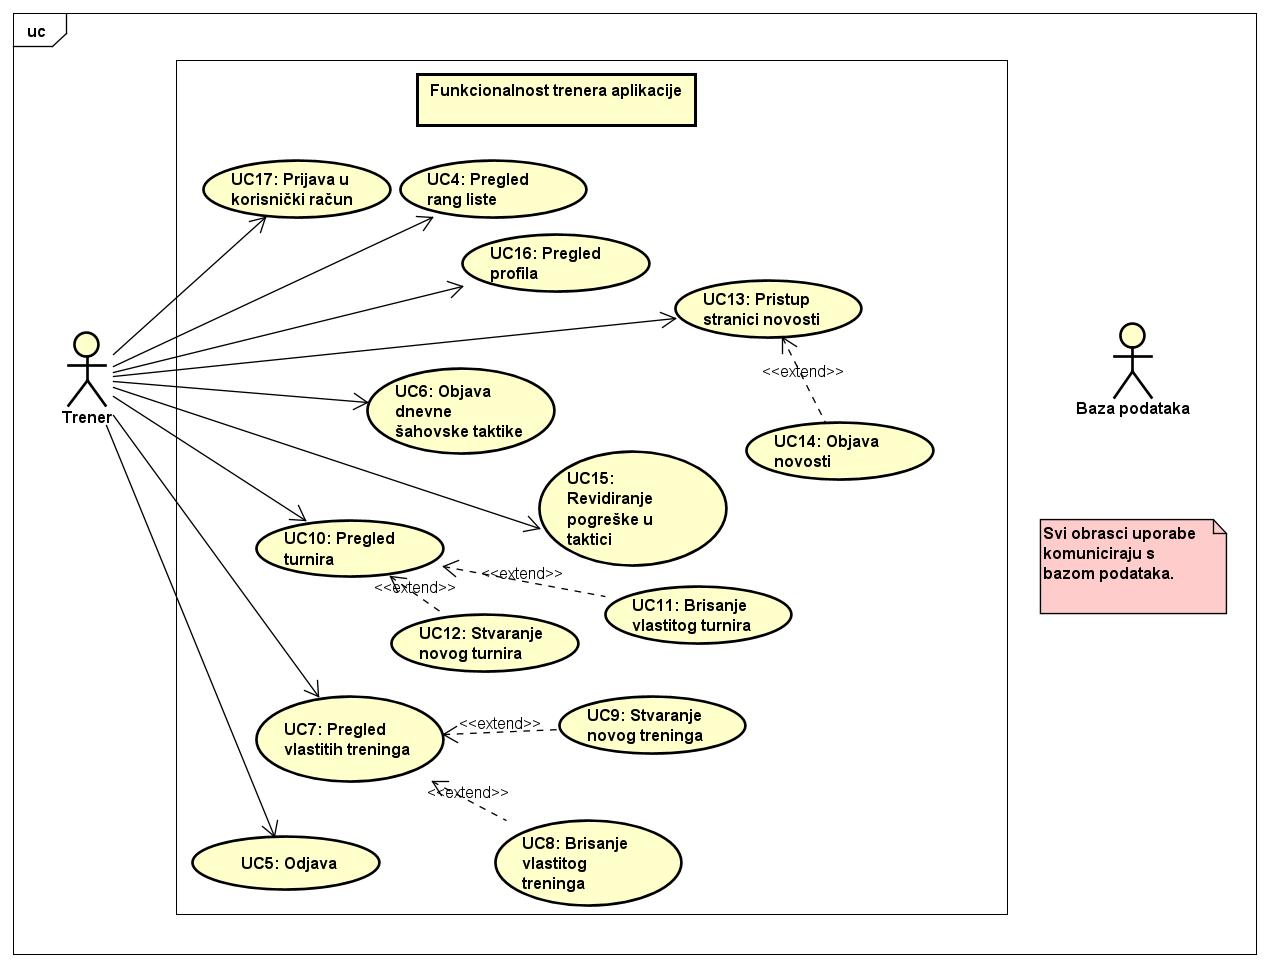
\includegraphics[scale=0.48]{dijagrami/UseCaseTrener.jpg} %veličina slike u odnosu na originalnu datoteku i pozicija slike
			\caption{Sekvencijski dijagram za UC$<$broj obrasca$>$}
			\label{fig:UC$<$broj obrasca$>$}
		\end{figure}
		
		\eject
				
			\subsection{Sekvencijski dijagrami}
			
			
				\textbf{Obrazac uporabe UC$<$broj obrasca$>$ - Stvaranje novog treninga}\\
				Trener šalje zahtjev web aplikaciji za stvaranje novog treninga. Web aplikacija dohvaća iz baze podataka sve ostale treninge tog trenera i provjerava da se novi trening ne preklapa ni sa jednim postojećim treningom. Ako uistinu ne postoji preklapanje, novi trening se zapisuje u bazu podataka te se treneru šalje obavijest o uspjehu kreiranja novog treninga. Ukoliko postoji preklapanje s već postojećim treningom, treneru web aplikacija javlja informacije o preklapanju i nemogućnosti stvaranja zatraženog treninga.
				\eject
				
				\begin{figure}[H]
					\centerfloat
        					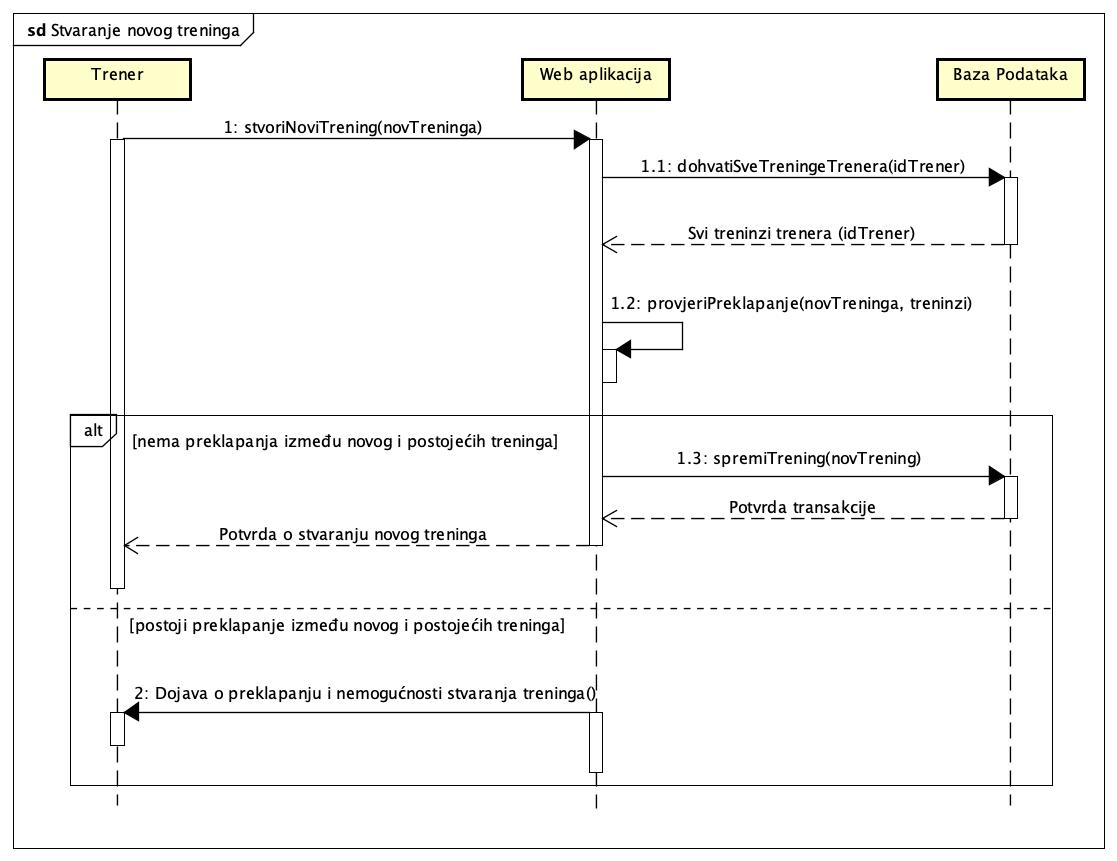
\includegraphics[scale=0.48]{dijagrami/StvaranjeNovogTreninga.jpg} %veličina slike u odnosu na originalnu datoteku i pozicija slike
        					\caption{Sekvencijski dijagram za UC$<$broj obrasca$>$}
        					\label{fig:UC$<$broj obrasca$>$}
				\end{figure}
				
				\eject
				
				\textbf{Obrazac uporabe UC$<$broj obrasca$>$ - Revidiranje pogreške u taktici}\\
				\\Trener šalje zahtjev za prikaz određene dojave o pogrešci taktike kako bi ju mogao pobliže proučiti i odlučiti je li primjedba valjana. Poslužitelj zatraženu dojavu vadi iz baze podataka te ju prikazuje. Taj prikaz sastoji se od osnovnih informacija o dojavi poput ime prijavljenje taktike, težine prijavljenje taktike itd., ali se sastoji i od simulacije dvije šahovske ploče. Na prvoj ploča simulira se trenutni tijek taktike, a na drugoj se simulira novi tijek taktike koji je predložen u dojavi o pogrešci. Trener pritiskom na odgovarajuće gumbe šalje zahtjeve za sljedeći korak u simulaciji. Trener također može i poslati zahtjev za resetiranje simulacije i tako ju vratiti u početni položaj. Nakon što je proučio simulaciju trener šalje poslužitelju zahtjev za potvrdu ili odbacivanje dojave o pogrešci. Ako je trener potvrdio dojavu, poslužitelj ju tako mora obilježiti u bazi podataka, te zatim oduzeti odgovarajući broj bodova svim igračima koji su uspješno riješili 'zastarjelu' verziju taktike. Ako je trener odbacio dojavu, poslužitelj ju samo mora evidentirati kao odbačenu u bazi podataka.
			

				
				\begin{figure}[H]
					\centerfloat
        					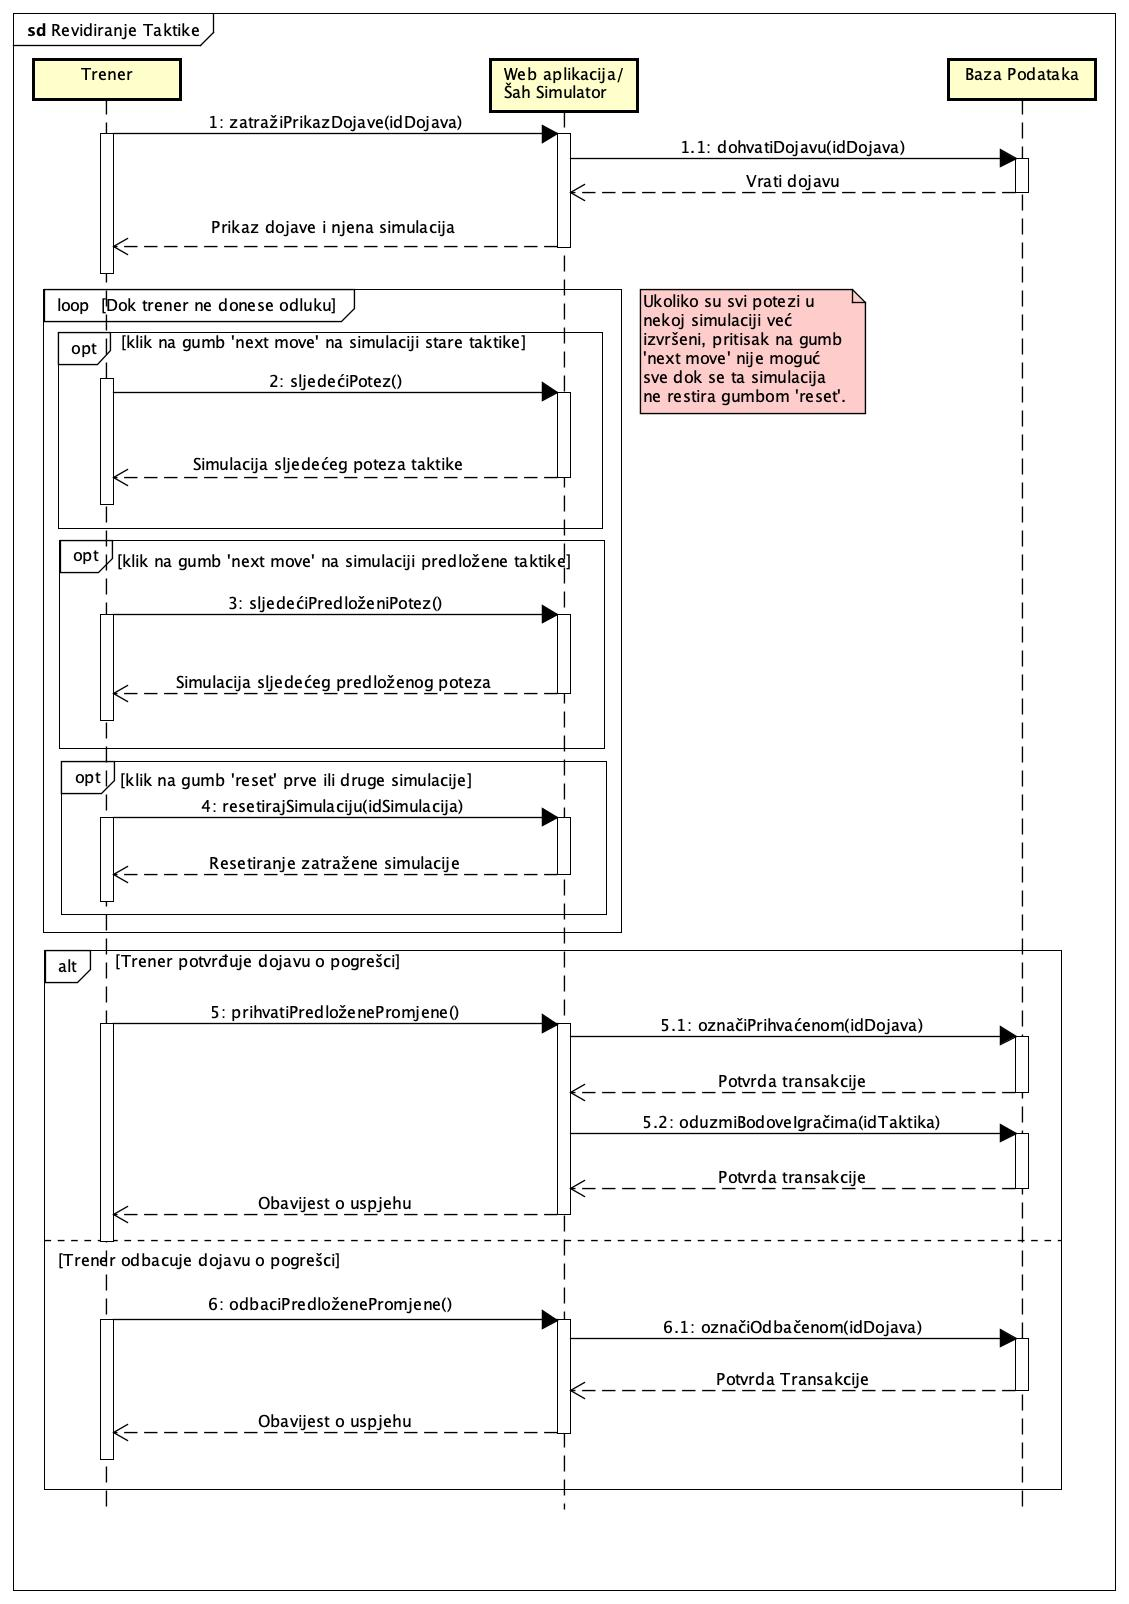
\includegraphics[scale=0.46]{dijagrami/RevidiranjeTaktike.jpg} %veličina slike u odnosu na originalnu datoteku i pozicija slike
        					\caption{Sekvencijski dijagram za UC$<$broj obrasca$>$}
        					\label{fig:UC$<$broj obrasca$>$}
				\end{figure}
				
				\eject
	
		\section{Ostali zahtjevi}
		
			\textbf{\textit{dio 1. revizije}}\\
			
			\textit{Nefunkcionalni zahtjevi i zahtjevi domene primjene dopunjuju funkcionalne zahtjeve. Oni opisuju \textbf{kako se sustav treba ponašati} i koja \textbf{ograničenja} treba poštivati (performanse, korisničko iskustvo, pouzdanost, standardi kvalitete, sigurnost...). Primjeri takvih zahtjeva u Vašem projektu mogu biti: podržani jezici korisničkog sučelja, vrijeme odziva, najveći mogući podržani broj korisnika, podržane web/mobilne platforme, razina zaštite (protokoli komunikacije, kriptiranje...)... Svaki takav zahtjev potrebno je navesti u jednoj ili dvije rečenice.}
			
			Sustav mora osigurati da odgovor na svaki zahtjev dođe unutar 5 sekundi. Sustav mora isto tako osiguravati da korisnici imaju sigurne šifre za svoje korisničke račune kako bi što bolje poboljšao sigurnost sustava. Sustav mora osigurati da svaka osoba ima samo jednu ulogu u aplikaciji. Sustav mora osigurati da korisnici ne mogu raditi ilegalne poteze u šahu.\\
			Sustav mora osigurati da korisnik mora unijeti sve potrebne podatke. \\
			Treneri prilikom stvaranja novog turnira mora unijeti naziv, datum i vrijeme početka te opis turnira. Treneri prilikom stvaranja novog termina treninga ne smije unijeti vrijeme koje mu je već zauzeto drugim terminom. Trener prilikom unosa nove novosti mora osigurati da novost ima naslov i sadržaj. \\
			Administrator prilikom stvaranja novog turnira mora unijeti naziv, datum i vrijeme početka, opis turnira te mora navesti trenera kojeg će sustav prepoznati kao organizatora turnira, pošto će tom treneru biti dane organizatorske ovlasti nad turnirom. Administrator prilikom stvaranja novog termina treninga mora navesti trenera kojem stvara termin te ne smije unijeti vrijeme koje je tom treneru već zauzeto drugim terminom.\\
			Član mora prilikom prijave pogreške u dnevnoj taktici mora unijeti poteze koje smatra ispravnim te opis tih poteza.\\
			Sustav mora mjeriti svakom članu vrijeme potrebno za rješavanje dnevne taktike te koristeći izmjereno vrijeme i ocjenu težine taktike dodijeliti članu bodove za tu taktiku. Sustav na bazi zbroja svih bodova, kreira težinsku listu rang listu članova.\\
			Korisničko sučelje će podržavati samo engleski jezik. Korisničko sučelje mora biti intuitivno za korištenje.\\
			
		 
			 
			 
			 
			 
	